\documentclass{beamer}
\beamertemplatenavigationsymbolsempty
\usepackage{graphicx}
\usepackage{listings}
\lstset{
    breaklines=true,
    numbers=left,
    numberstyle=\scriptsize,
    frame=leftline,
    basicstyle=\ttfamily}

% TODO
%  * use \begin{frame}[fragile] with code examples


\begin{document}
\begin{frame}

    {\LARGE Uvod do Bitcoinu}\\
    \vspace{7mm}
    {\Large Ondrej Sika \lstinline|<ondrej@ondrejsika.com>|}\\
    \vspace{7mm}
    {\large Slush Pool (\url{mining.bitcoin.cz})}\\
    \vspace{7mm}
    26. 8. 2015, Pilsen, Czech Republic\\

\end{frame}

\begin{frame}

    {\LARGE Co je Bitcoin}\\
    \vspace{5mm}
    {\LARGE Jak Bitcoin funguje}\\
    \vspace{5mm}
    {\LARGE Bitcoinove penezenky}\\
    \vspace{5mm}
    {\LARGE Kde koupim Bitcoiny}\\
    \vspace{5mm}
    {\LARGE Kde utratim Bitcoiny}\\

\end{frame}

\begin{frame}

    {\LARGE Co je Bitcoin}\\

    \vspace{5mm}

    - {\bf "digitalni zlato"}\\
    - peer to peer digital cash - neni nutny prostrednik pro transakce\\
    - distribuovany - ulozen v mnoha kopiich na celem svete\\
    - decentrializovany - nema centralni autoritu\\
    - "anonymni"\\

\end{frame}

\begin{frame}

    {\LARGE Vyhody}\\

    \vspace{5mm}

    - decentralizovany, distribuovany\\
    - nikdo vam nemuze zmrazit ucet\\
    - "anonymni"\\

    \vspace{10mm}

    {\LARGE Nevyhody}\\

    \vspace{5mm}

    - nemuzete zrusit platbu\\
    - nachylnost ke kradezim\\
    - spojovan s nelegalni cinnosti - silkroad\\
    - "anonymni"\\

\end{frame}

\begin{frame}

    {\LARGE Jak Bitcoin funguje}\\

    \vspace{5mm}

    - zalozeno na cryptografickych zakladech\\
    - transakce je podepsany prikaz k prevodu penez konkretni penezenkou (privatni klic) na jinou penezenku (verejny klic)\\
    - transakce jsou ukladany do blockchainu, posloupnost bloku transakci bez nutnosti centralni autority\\
    - mining - generovani novych coinu a bloku transakci - zajistuje bezpecnost site\\

\end{frame}

\begin{frame}

    {\LARGE Bitcoinove penezenky}\\

    \vspace{5mm}

    \url{https://bitcoin.org/en/choose-your-wallet}

    \vspace{5mm}

    - hardwarove - Trezor\\
    - PC - Bitcoin Qt, Electrum\\
    - mobilni - Mycelium, Coinbase\\
    - web - Coinbase\\
    - paperwallets\\

\end{frame}

\begin{frame}

    {\LARGE Trezor}\\

    \vspace{5mm}

    - Nejbezpecejsi zpusob ulozeni Bitcoinu\\
    - Podpora vice accountu (BIP32)\\
    - Online klient \url{https://mytrezor.com}\\
    - Podpora v Androin Myceliu\\
    - Vice na \url{http://bitcointrezor.com}\\
    - Produkt nasi spolecnosti (SatoshiLabs)\\

    \vspace{5mm}

    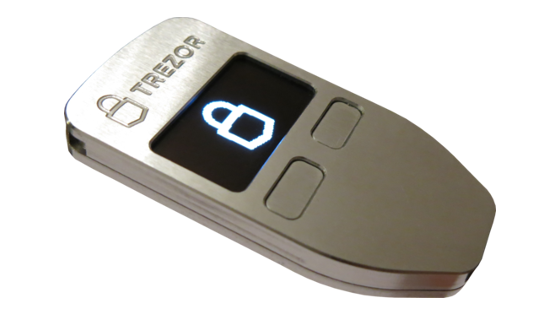
\includegraphics[scale=0.3]{img/trezor}

\end{frame}

\begin{frame}

    {\LARGE Bitcoin Qt}\\

    \vspace{5mm}

    - oficialni Bitcoin penezenka\\
    - vyhoda - bez zavislosti tretich stran\\
    - nevyhoda - stahuje cely blockchain (50GB)\\
    - \url{https://bitcoin.org/en/download}

    \vspace{10mm}

    {\LARGE Electrum}\\

    \vspace{5mm}

    - vyhoda - nemusi mit stazeny blockchain\\
    - nevyhoda - nutnost pouzivat servery treti strany\\
    - \url{https://electrum.org}

\end{frame}

\begin{frame}

    {\LARGE Mycelium}\\

    \vspace{5mm}

    - podpora vice accountu (BIP32)\\
    - Android verze podporuje trezor\\
    - privatni klice jsou pouze v telefonu\\
    - backup seed\\
    - \url{https://mycelium.com/bitcoinwallet}\\

    \vspace{10mm}

    {\LARGE Coinbase}\\

    \vspace{5mm}

    - web + mobilni aplikace\\
    - coiny ulozene na adresach v Coinbase (uzivatel nema pristup k privatnim klicum)\\
    - jeden ucet na webu i v mobilu\\
    - \url{https://coinbase.com}\\

\end{frame}

\begin{frame}

    {\LARGE Paper wallet}\\

    \vspace{5mm}

    - klice jsou vytisteny na papir (QR kody)\\
    - hodene online generatoru: \url{http://paperwallet.net}\\

    \vspace{5mm}

    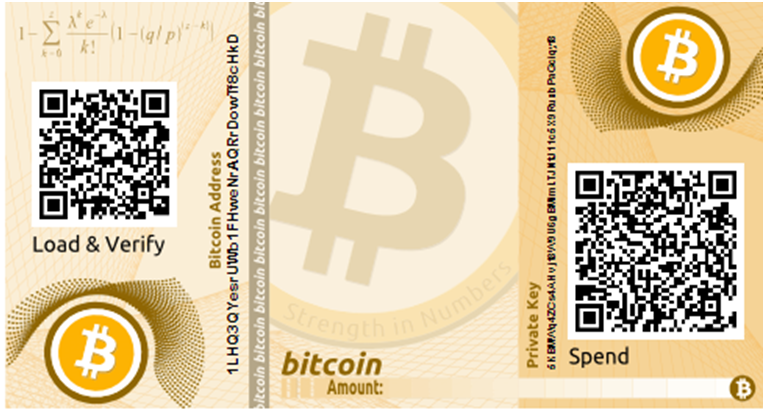
\includegraphics[scale=0.3]{img/paperwallet}

\end{frame}

\begin{frame}

    {\LARGE Kde koupim Bitcoiny}\\

    \vspace{5mm}

    - u me\\
    - localbitcoins.com\\
    - Bitcoin ATM\\
    - burzy: Bitstamp, Kraken, ...\\

\end{frame}

\begin{frame}

    {\LARGE localbitcoins.com}\\

    \vspace{5mm}

    - prodej i nakup BTC za lokalni menu (CZK)\\
    - rychle\\
    - relativne bezpecne\\

\end{frame}

\begin{frame}

    {\LARGE Bitcoin ATM}\\

    \vspace{5mm}

    - v Plzni: Vedeckotechnicky park (Borska pole) - pouze nakup BTC\\
    - v Praze jsou i obousmerne\\
    - kurz + 3 - 10\% proti burzam\\

    \vspace{5mm}

    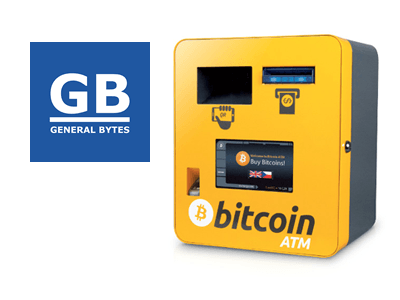
\includegraphics[scale=0.4]{img/atm}

\end{frame}

\begin{frame}

    {\LARGE Kde utratim sve Bitcoiny}\\

    \vspace{5mm}

    - Online: Amazon, Dell, SAS (Airlines), ...\\
    - Offline: Seraf, \url{https://Coinmap.org}\\

\end{frame}

\begin{frame}

    {\LARGE Coinmap.org}\\

    \vspace{5mm}

    - vetsina mist kde prijimaji Bitcoin\\
    - vice nez 8 000 mist po svete\\

    \vspace{5mm}

    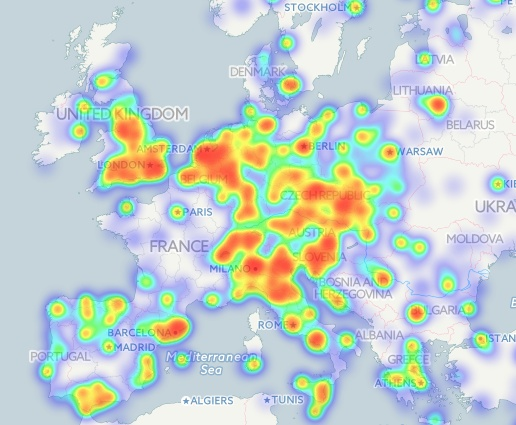
\includegraphics[scale=0.4]{img/coinmap}

\end{frame}

\begin{frame}

    {\LARGE Uzitecne odkazy}\\

    \vspace{5mm}

    - oficialni web Bitcoinu - \url{https://bitcoin.org/}\\
    - prochazeni blockchainu - \url{https://blockchain.info/}\\
    - grafy ceny Bitcoinu - \url{https://bitcoinwisdom.com/}\\
    - web Satoshilabs (nase firma) - \url{https://satoshilabs.com}\\
    - ceska BTC komunita - \url{https://fb.com/groups/bitcoincz/}\\

\end{frame}

\begin{frame}

    {\LARGE Dekuji za poroznost \& Otazky \& Diskuze}\\

    \vspace{1cm}

    \texttt{ondrej@ondrejsika.com}\\
    \url{http://ondrejsika.com}\\
    \texttt{@ondrejsika}\\

    \vspace{1cm}

    Sources:\\
    \url{http://url.os1.cz/uvod-do-bitcoinu/}
\end{frame}

\end{document}

